% Part 1: Determining RecB binding time
\section*{Results}

\subsection*{RecB forms long-lived spots when recruited to cipro\-floxacin DSBs}

\begin{figure*}[htbp]
    \centering
    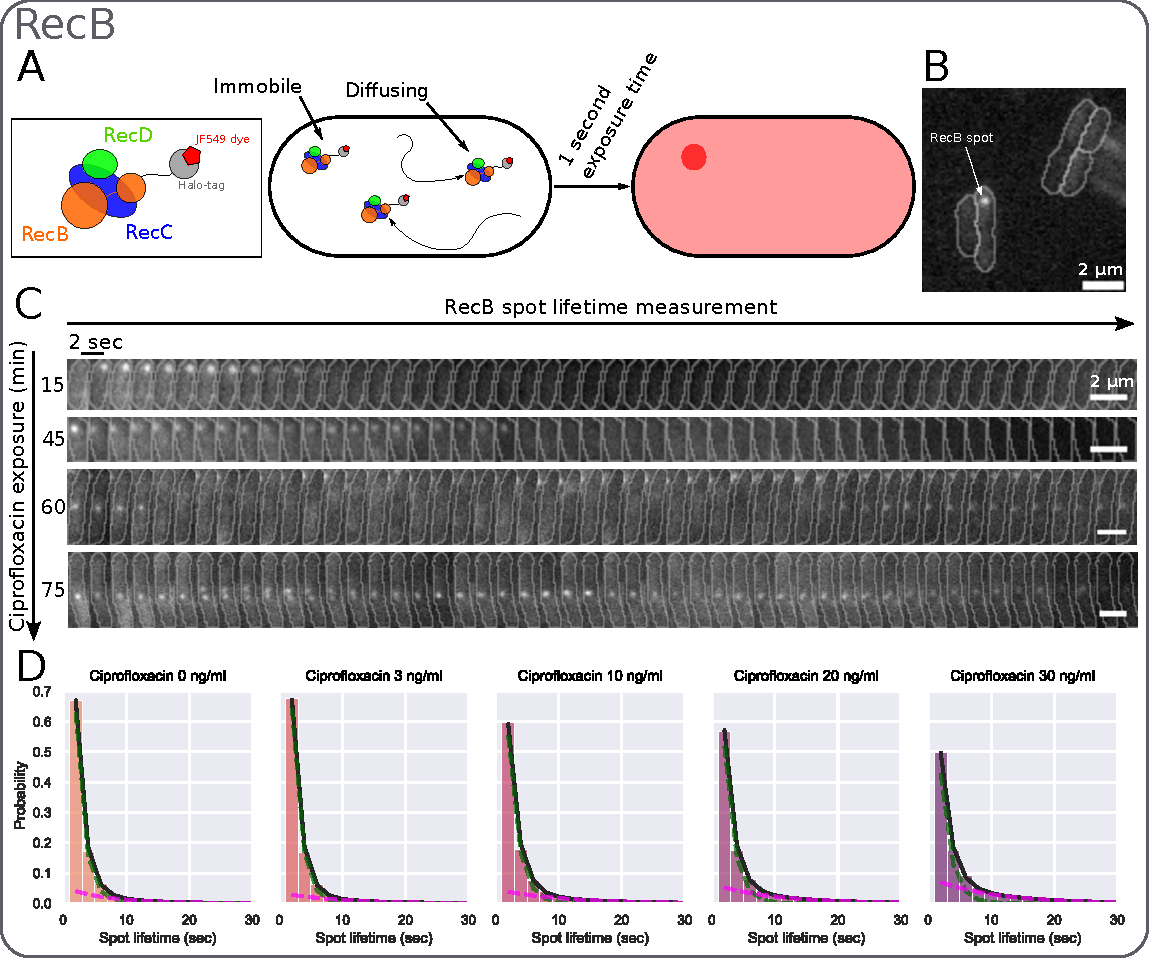
\includegraphics[width=.8\textwidth]{Figures/Fig1_RecB_lifetime.pdf}
    \caption{Measuring the binding time of RecB on DNA. \textbf{(A)} Scheme of our experimental protocol. The RecB subunit of the RecBCD complex is fused to a Halo-tag, bound by the JF549 fluorescent dye\cite{Lepore2019a, Lepore2023}. A long exposure time (1 sec) makes diffusing molecules appear as diffuse signal in the cell, while DNA-bound molecules are visible as bright, diffraction-limited spots. \textbf{(B)} Example image of a RecB spot (white arrow). \textbf{(C)} Example kymographs of RecB throughout an acquisition. A short timelapse (100 sec) is acquired at a different position every 2 min for 75 min. \textbf{(D)} RecB spot lifetime histograms at 3, 10, 20 and 30 ng/ml ciprofloxacin (bars), fitted with a bi-exponential decay model (black line, fit components showed as dashed lines). \ncells{66,764}. \nspots{170,138}}
    \label{Fig:lifetimes}
\end{figure*}

To quantify RecB binding time to DNA in live \textit{E. coli}, we used a Halo-tag fusion to the RecB subunit, conjugated to the JF549 fluorescent dye (Figure \ref{Fig:lifetimes}A). The fusion was previously used and characterised, ensuring specific one-to-one labelling of RecB molecules without adverse effects on the DNA repair process.\cite{Lepore2019a,Lepore2023} To detect the binding of RecB to DSBs, we applied the previously developed technique of localisation enhancement.\cite{Yu2006, Elf2007} Since RecB is present at low copy numbers in \textit{E. coli} ($\sim$5 molecules per cell on average\cite{Lepore2019a}), imaging live cells with a long exposure time (1 second) made fast-diffusing RecB molecules appear as weak homogeneous signal in the cell, while slow-diffusing RecB molecules formed intense diffraction-limited spots (referred to throughout this article as RecB spots, Figures \ref{Fig:lifetimes}A and \ref{Fig:lifetimes}B). The complete absence of similar spots in cells expressing the free Halo-tag from a plasmid confirmed that these structures were specific to RecB (Supp. Figure \ref{SIFig:freehalo_image}). We observed RecB spots in cells that were not exposed to an exogenous source of DNA damage as expected, as these cells are still subject to occasional endogenous DNA damage, such as replication fork collisions which were previously reported to affect $\sim$18\% of cells per cell cycle.\cite{Sinha2018} We added ciprofloxacin to agar pads before imaging and acquired timelapse videos every 2 min for 60 min (Figure \ref{Fig:lifetimes}C), which allowed us to quantify RecB binding at different time points ranging from 15 to 75 min after the start of ciprofloxacin exposure.

%% RecB spot lifetime histograms change upon exposure to ciprofloxacin
%%% They are not well-fitted by a monoexponential decay (SI fig)
%%% We fit with a bi-exponential decay model
%%% Comment on lifetimes/populations, in table
%%% Fitting lifetimes on different timepoints (SI Fig) shows no change with duration of ciprofloxacin exposure
Using the timelapse data, we built histograms of RecB spot lifetimes at the different ciprofloxacin concentrations (Figure \ref{Fig:lifetimes}D). Fitting these histograms with a mono-exponential decay model ($y = a.e^{-k.t}$) did not match the experimental data accurately (Supp. Figure \ref{SIFig:monoexp_fits}). In particular, it did not account for a population of longer-lived RecB spots ($>$ 10 sec), which was more visible at the higher ciprofloxacin concentrations. Fitting with a bi-exponential decay model ($y = a_1.e^{-k_1.t} + a_2.e^{-k_2.t}$) accounted much better for the longer-lived RecB spots (Figure \ref{Fig:lifetimes}D). The bi-exponential fit outlined two populations of spots with different lifetimes: a short-lived one, with lifetimes ranging from 1.4 to 1.7 sec, and a longer-lived one, with lifetimes ranging from 10 to 14 sec (Table \ref{tab:fit_results}). Even though the short-lived spots always represented a majority of events (over 90\% of the spots), the proportion of long-lived spots tended to increase under higher ciprofloxacin exposure (from 1.4\% $\pm$ 0.3 under 3 ng/ml ciprofloxacin to 5.5\% $\pm$ 1.4 under 30 ng/ml ciprofloxacin). To test whether the duration of ciprofloxacin exposure had an effect on spot lifetimes, we performed separate fits for 15-min windows in all experiments (Supp. Figure \ref{SIFig:RecB_lifetimes_timepoints}). Although lifetime determination was less precise due to the smaller amount of data for each fit, spot lifetimes did not change between the beginning and the end of our experiments.

\begin{table}[htbp]
    \centering
    \caption{Parameters derived from the spot lifetime histogram fits (Figures \ref{Fig:lifetimes}D and \ref{Fig:recruitment}B). The lifetime was calculated as the inverse of the fitted dissociation rate. Values are given as the median $\pm$ standard deviation over at least 3 independent datasets. \ncells{66,764}. \nspots{170,138}}
    \begin{tabular}{llll}
        \toprule
         &  & Lifetime (sec) & Population (\%) \\
        Ciprofloxacin & Type &  &  \\
        \midrule
        \multirow[t]{2}{*}{0 ng/ml} & Short & 1.4 $\pm$ 0.2 & 98.2 $\pm$ 1.0 \\
         & Long & 9.5 $\pm$ 9.7 & 1.8 $\pm$ 1.0 \\
        \cline{1-4}
        \multirow[t]{2}{*}{3 ng/ml} & Short & 1.5 $\pm$ 0.1 & 98.6 $\pm$ 0.3 \\
         & Long & 10.5 $\pm$ 1.3 & 1.4 $\pm$ 0.3 \\
        \cline{1-4}
        \multirow[t]{2}{*}{10 ng/ml} & Short & 1.7 $\pm$ 0.2 & 97.6 $\pm$ 0.6 \\
         & Long & 13.7 $\pm$ 2.3 & 2.4 $\pm$ 0.6 \\
        \cline{1-4}
        \multirow[t]{2}{*}{20 ng/ml} & Short & 1.6 $\pm$ 0.2 & 96.6 $\pm$ 0.8 \\
         & Long & 11.8 $\pm$ 2.1 & 3.4 $\pm$ 0.8 \\
        \cline{1-4}
        \multirow[t]{2}{*}{30 ng/ml} & Short & 1.7 $\pm$ 0.2 & 94.5 $\pm$ 1.4 \\
         & Long & 13.3 $\pm$ 2.2 & 5.5 $\pm$ 1.4 \\
        \cline{1-4}
        \bottomrule
        \end{tabular}
    \label{tab:fit_results}
\end{table}

%% To check what these two populations are, we use the Gam protein to prevent DNA binding and fit with the same model
%% We are unable to assign short DNA binding events, but we can confidently detect longer DNA binding events
To determine whether both short- and long-lived spots resulted from RecB binding to DNA, we measured RecB spot lifetime in the presence and absence of ciprofloxacin while over-expressing the Gam protein of phage $\lambda$ from a plasmid. The Gam protein was previously shown to bind in place of DNA on the RecBCD complex\cite{Wilkinson2016}, and its overexpression is expected to abolish RecBCD binding to DNA. Accordingly, cells that over-expressed Gam and were exposed to high ciprofloxacin (30 ng/ml) showed little elongation compared to cells that did not overexpress Gam (Supp. Figure \ref{SIFig:Gam_cell_length}), indicating that most cells did not induce the SOS response, due to the inability of the RecBCD-Gam complex to bind to DSBs. The resulting RecB spot lifetime histograms showed a near-complete disappearance of the long-lived spots, while short-lived ones were still present (Supp. Figure \ref{SIFig:Gam_RecB_lifetimes_fits}). This was confirmed by fitting the histogram with our bi-exponential decay model, which found a proportion of long-lived spots (1.4\% $\pm$ 0.5) similar to wild-type cells that were not exposed to ciprofloxacin (1.8\% $\pm$ 1, Table \ref{tab:fit_results}). The residual amount of long-lived RecB spots in the presence of Gam could be due to residual DNA binding despite the presence of Gam. This residual binding could also be the cause for the small increase in cell length observed in Gam-expressing cells under 30 ng/ml ciprofloxacin (Supp. Figure \ref{SIFig:Gam_cell_length}). Since Gam overexpression prevents RecB binding to DNA ends, and specifically caused long-lived spots to disappear, we can conclude that long-lived spots correspond to RecB molecules that have bound to DNA ends. Given that under Gam overexpression, 95\% of RecB spots were shorter than 10 sec (Figure \ref{Fig:recruitment}A), we considered any spot with a lifetime over 10 sec to be a DNA-bound RecB molecule. The nature of short-lived spots is more difficult to determine, and might be a combination of short-lived DNA binding, and slow diffusion of the RecBCD-Gam-Halo complex (Supp. Note \ref{note:spurious_spots} and Supp. Figure \ref{SIFig:displacement_simul}). Therefore, spots that are visible only for a few seconds cannot be reliably assigned as either DNA-bound or freely diffusing.

\begin{figure}[htbp]
    \centering
    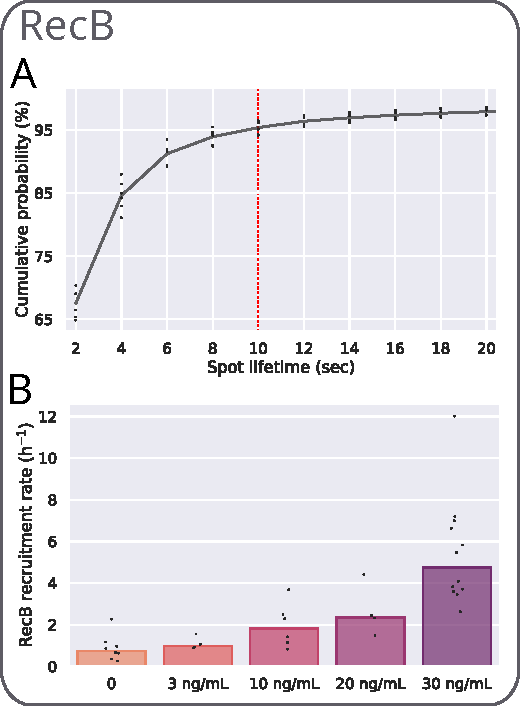
\includegraphics[width=.4\textwidth]{Figures/Fig2_RecB_recruitment.pdf}
    \caption{RecB DNA binding under ciprofloxacin exposure. \textbf{(A)} Probability of a spot corresponding to a DNA-bound RecB molecule, for cells over-expressing the Gam protein. Black dots show individual datasets, the black line is the average between them, and the red dashed line shows the smallest lifetime at which RecB spots have 95\% probability to be DNA-bound. \ncells{8,812}. \nspots{18,698} \textbf{(B)} Recruitment rate of RecB on DNA at different ciprofloxacin concentrations. Black points show individual datasets, and bars the median value. \ncells{66,764}. \nspots{170,138}}
    \label{Fig:recruitment}
\end{figure}

%% We use the number of spots and proportion of long-lived spots to estimate the rate of recruitment of RecB on the DNA
Whereas the lifetime of the fluorescent spots informs us on how long RecB stays bound to DNA, the rate of appearance of spots helps us estimate the rate of recruitment of RecB to DSBs under each DNA damage condition (Figure \ref{Fig:recruitment}B). We estimated that under endogenous damage or low ciprofloxacin concentrations, 1 to 2 RecB molecules are recruited to the DNA per hour on average. This is roughly consistent with the previous estimate of 18\% of cells generating an endogenous DSB per cell cycle\cite{Sinha2018}. At ciprofloxacin concentrations above the MIC (30 ng/ml), the recruitment rate increased sharply to an average of 5 RecB recruited per hour. Furthermore, we expect that this recruitment rate gives a close estimate of the rate of formation of DSBs (see discussion).

% Part 2: Effects of DSBs and the repair process on the cell
\subsection*{Ciprofloxacin exposure induces formation of RecA filaments and nucleoid compaction}

\begin{figure*}[htbp]
    \centering
    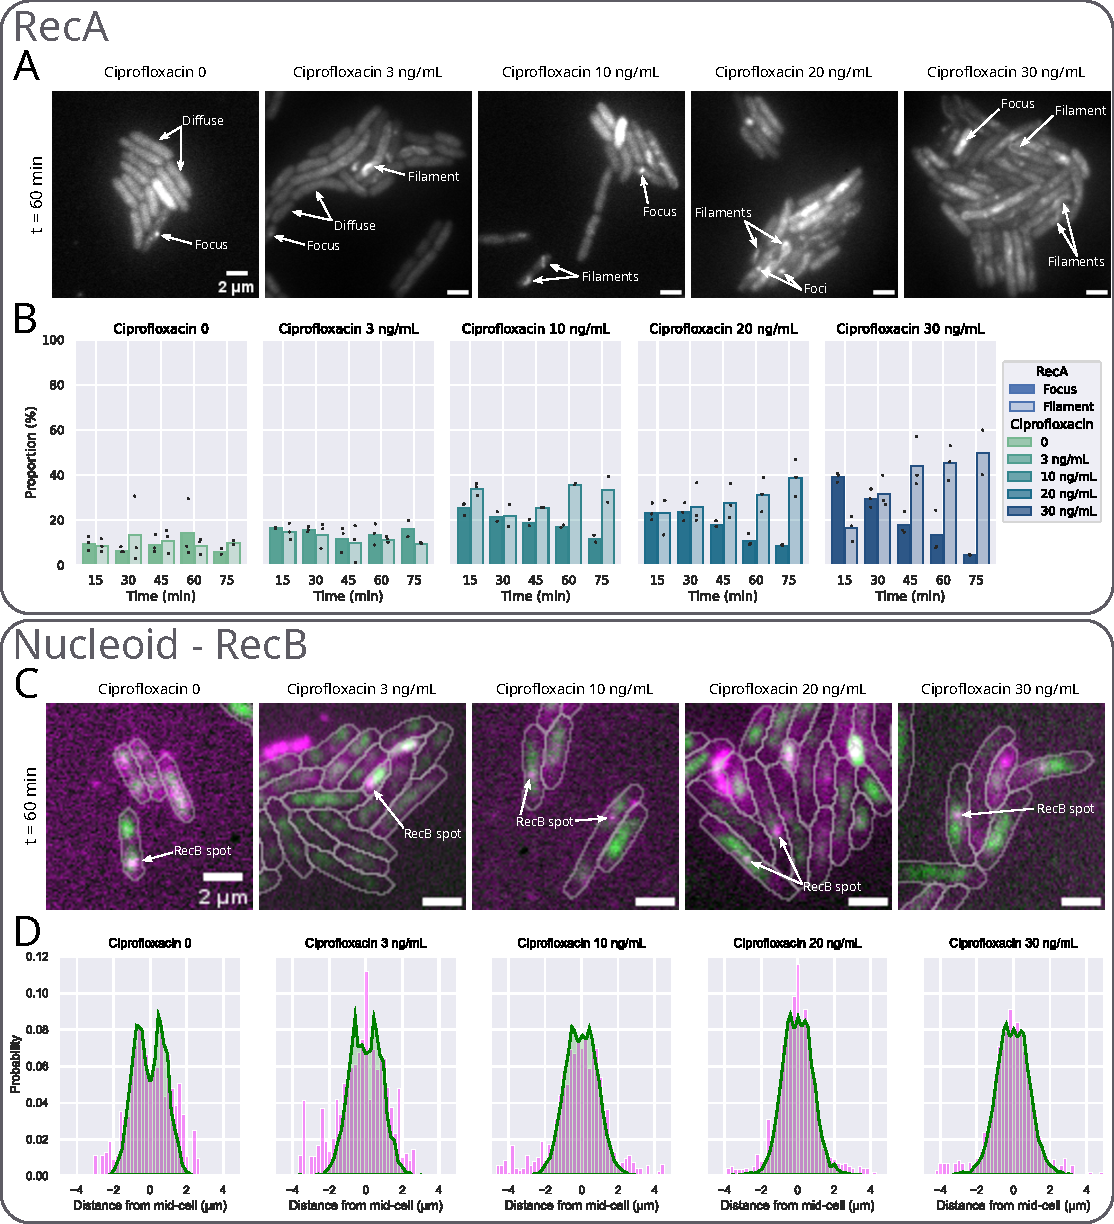
\includegraphics[width=.8\textwidth]{Figures/Fig3_cell_response.pdf}
    \caption{Bacterial cell response to the induction of DSBs by ciprofloxacin. \textbf{(A)} Representative images of cells containing different RecA structures (diffuse fluorescence, foci or filaments) after 60 minutes of exposure to ciprofloxacin. Arrows point to representative examples of each of these structures. \textbf{(B)} Proportion of cells containing RecA foci or filaments. Black dots represent individual datasets, and bars the average between them. \ncells{32,031}. \textbf{(C)} Representative images of cells (segmented outline in grey) showing the nucleoid (green) and RecB-associated fluorescence (magenta). RecB spots (indicated by arrows) are located in close proximity to the nucleoid. \textbf{(D)} Overlay of nucleoid density (green area) and position of DNA-bound RecB molecules (magenta bars) along the cell's long axis, for different ciprofloxacin concentrations (0 to 30 ng/ml). \ncells{24,014}. \nspots{79,969}. \nnucl{31,441}.}
    \label{Fig:reca_nucleoid}
\end{figure*}

%% RecA imaging
During processing of DSBs, RecBCD facilitates the loading of the RecA protein on single-stranded DNA. To broaden our view of the repair process downstream of RecBCD, we imaged a tandem fusion of RecA with the fluorescent protein SYFP2.\cite{Wiktor2021} Based on the fluorescence distribution in the cells (Figure \ref{Fig:reca_nucleoid}A), we identified three states of RecA: diffuse, forming a bright focus, or forming an elongated filament, which matches previous \emph{in-vivo} observations of RecA\cite{Wiktor2021}. Because of the large diversity of shapes observed, especially for RecA filaments, the detection of RecA structures by rule-based algorithms was challenging. Therefore, we designed and trained a deep-learning algorithm capable of classifying individual cells based on the three types of structures cited above (Figure \ref{Fig:reca_nucleoid}B, Supp. Figure \ref{SIFig:object_class}). In cells that were not exposed to ciprofloxacin, the RecA-associated fluorescence was mostly diffuse, and occasionally formed a bright focus. This is consistent with cells undergoing occasional endogenous DNA damage. The proportion of cells that contained RecA filaments was low in the absence of ciprofloxacin ($\sim$10\%). After one hour of exposure, the proportion of cells that contained a RecA filament had increased to $\sim$40\% at 20 ng/ml ciprofloxacin, and $\sim$60\% at 30 ng/ml. RecA foci on the other hand formed quickly following ciprofloxacin exposure (present in $\sim$40\% of the cells after 15 min of exposure to 30 ng/ml ciprofloxacin) and came back to endogenous damage level after $\sim$1 hour. Taken together, these results show that RecA foci are transient structures in the repair process that do not accumulate under high DNA damage, whereas RecA filaments accumulate under constant exposure to ciprofloxacin. This accumulation could be due to cells undergoing high levels of DNA damage, with several DSBs occuring over the course of the experiment (Figure \ref{Fig:recruitment}B). In these conditions, it would become increasingly likely for all copies of a locus to be damaged, and the DSB repair pathway to be stuck at the step of homology searching.

%% We imaged nucleoid and RecB in the same experiment
%% Ciprofloxacin exposure causes nucleoid compaction and centring
In \emph{E. coli}, the loading of RecA on DNA triggers the SOS response, which inhibits cell division, leading to cell filamentation. Previous studies have reported that the SOS response also triggers compaction of the bacterial nucleoid.\cite{Odsbu2014} To see if this was the case for breaks induced by ciprofloxacin in our experimental conditions, we stained DNA using the Sytox Green dye. The use of a green dye allowed us to concomitantly image RecB, and to correlate the position of DNA-bound RecB molecules with that of the nucleoid. Figure \ref{Fig:reca_nucleoid}C shows representative images of the nucleoid and DNA-bound RecB after 60 minutes of exposure to different concentrations of ciprofloxacin. In untreated cells, the nucleoid was often observed to be bi-lobed, consistently with previous observations\cite{Lepore2023}. Upon exposure to ciprofloxacin, the cells appeared elongated, and the nucleoid was often compacted in the centre of the cell. As a result of the nucleoid compaction, the total fraction of the cell occupied by the nucleoid decreased, from 40\% on average in untreated cells to 31\% in cells exposed to 30 ng/ml of ciprofloxacin for an hour (Supp. Figure \ref{SIFig:nucleoid_compaction}). This compaction was accompanied by a centring of the nucleoid along the cell's long axis. Supp. Figure \ref{SIFig:nucleoid_position} shows that upon increasing exposure to ciprofloxacin (in time and concentration), the cells elongate, and nucleoids were increasingly centred.

%% Nucleoid and RecB position are correlated
%% Interpretation: RecB spot centring is due to nucleoid centring
As expected, DNA-bound RecB were found in close proximity to the nucleoid (Figure \ref{Fig:reca_nucleoid}C). Figure \ref{Fig:reca_nucleoid}D shows the strong overlap between the spatial distribution of DNA-bound RecB spots and the nucleoid density in the cell (Supp. Figure \ref{SIFig:recb_nucleoid_timepoints} shows the same data after different durations of ciprofloxacin exposure). Due to nucleoid compaction and centring, both the nucleoid density and the position of DNA-bound RecB remained within $\sim$2 µm either side of the cell centre, despite the cells having elongated significantly.

% Part 3: Mutants in the repair pathway
\subsection*{RecB dissociation does not depend on RecA loading}

\begin{figure*}[htbp]
    \centering
    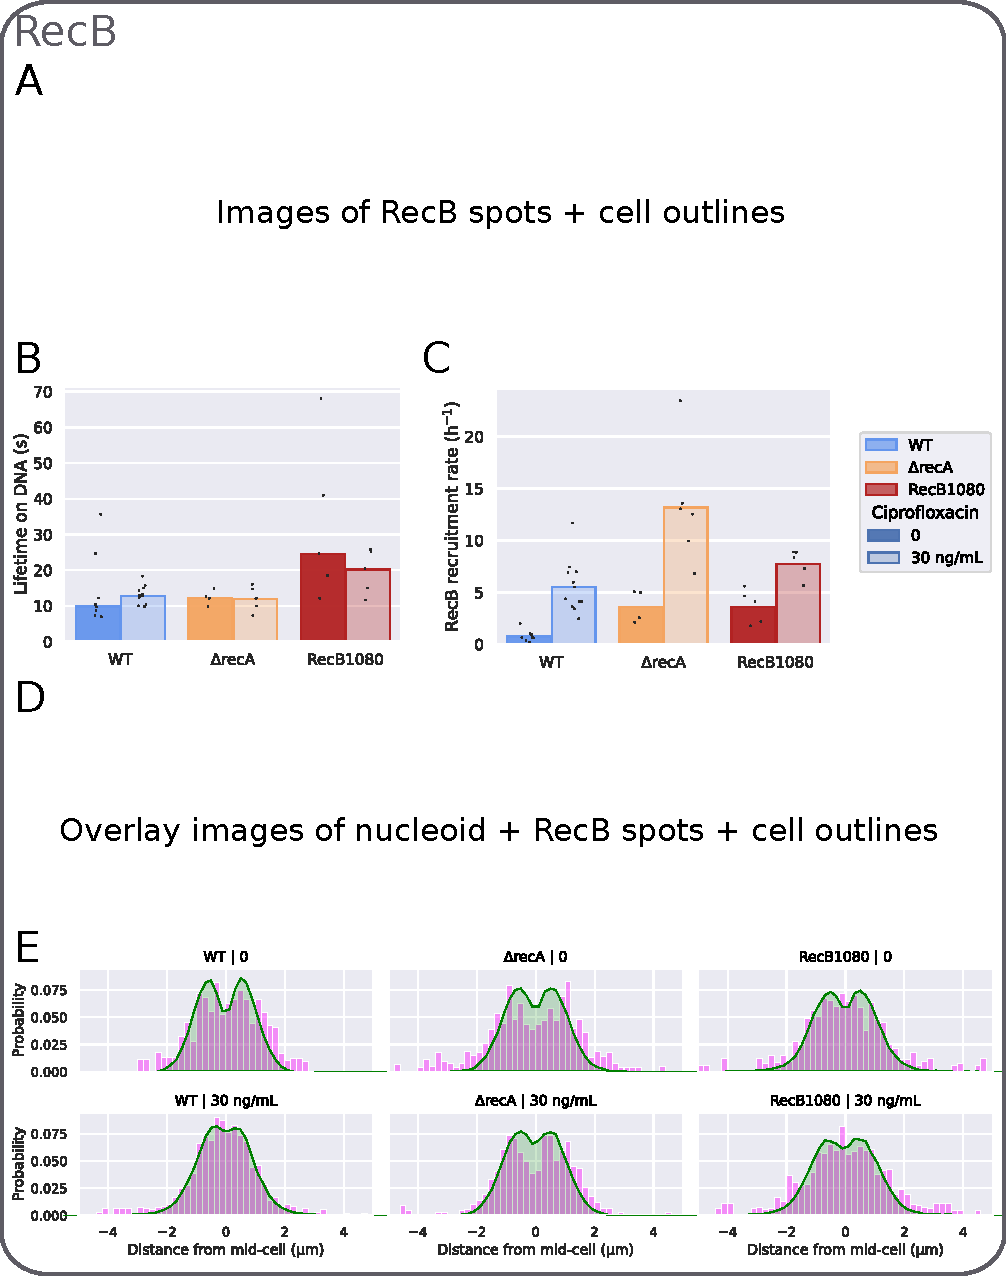
\includegraphics[width=.75\textwidth]{Figures/Fig4_mutants.pdf}
    \caption{RecB binding to DNA in the \dreca\ and \teneighty\ mutant strains in the absence and presence of ciprofloxacin (30 ng/ml). \textbf{(A)} Representative brightfield images of wild-type (WT), \dreca\ and \teneighty\ mutants cells, in the presence and absence of ciprofloxacin (30 ng/ml). \textbf{(B)} Fitted lifetimes of RecB molecules on DNA. Black dots show individual datasets, and bars the median values. \ncells{56,131}. \nspots{177,646}. \textbf{(C)} Rate of recruitment of RecB to the DNA. Black dots show individual datasets, and bars the median values. \ncells{56,131}. \nspots{177,646}. \textbf{(D)} Representative overlay images of RecB-associated fluorescence (magenta) and the bacterial nucleoid (green). Segmented cell outline shown in grey. \textbf{(E)} Overlay of nucleoid density (green area) and position of DNA-bound RecB molecules (magenta bars) along the cell's long axis. \ncells{15,029}. \nspots{58,331}. \nnucl{20,831}.}
    \label{Fig:mutants}
\end{figure*}

%% Effect of ciprofloxacin exposure on the different mutants
Imaging RecB binding to DSBs in the presence of different concentrations of ciprofloxacin allowed us to determine that the amount of DNA damage experienced by the cells did not influence the time spent by RecB on DNA. Next, we wanted to test whether RecB dissociation from DNA was influenced by RecA loading. Therefore, we imaged the \dreca\ and \teneighty mutants in the presence and absence of 30 ng/ml ciprofloxacin. Figure \ref{Fig:mutants} shows brightfield images of cells that were not exposed to ciprofloxacin, and cells that were exposed to 30 ng/ml ciprofloxacin for 60 min. Supp. Figure \ref{SIFig:mutants_cell_lengths} shows the average cell lengths in the different conditions and ciprofloxacin exposure durations. As previously observed, wild-type cells show a clear response to exposure to 30 ng/ml ciprofloxacin, where the cell length increases significantly due to induction of the SOS response. In contrast to this, since the \dreca\ mutant is unable to form a RecA filament, it is also unable to induce the SOS response. Cell length therefore remains unchanged, even upon prolonged exposure to 30 ng/ml ciprofloxacin. In the absence of ciprofloxacin, the \teneighty\ mutant cells were slightly more elongated than wild-type cells. This matches previous indications that this mutant has a higher baseline of SOS induction than wild-type cells in the absence of exogenous DNA damage\cite{Lepore2023}. Upon exposure to ciprofloxacin, the cell length of the \teneighty\ mutant increased, albeit slightly less on average than the wild-type's (Supp. Figure \ref{SIFig:mutants_cell_lengths}). This might be a reflection of \teneighty's inability to directly load RecA on the DNA, and the use of the alternative RecFOR pathway leading to a weaker or delayed SOS response\cite{Ivancic-Bace_2003,Lepore2023}.

%% DNA binding lifetimes
As for the wild-type strain, we computed histograms of RecB spot lifetimes, and fitted them with a bi-exponential decay model (Supp. Figure \ref{SIFig:mutants_biexp_fits}), from which we extracted the binding times of RecB on DNA (Figure \ref{Fig:mutants}B). In the \dreca\ mutant, the DNA-binding lifetime of RecB was similar to the wild-type ($\sim$10 sec). This suggests that RecA loading by RecBCD does not play a role in triggering the dissociation of RecBCD from DNA. Both in the presence and absence of ciprofloxacin, \teneighty\ stayed bound to DNA for longer than wild-type RecB ($\sim$20 sec). This could be due to the inability of \teneighty\ to digest the DNA it unwinds, making dissociation more challenging due to the DNA strands threading through the RecBCD complex.

%% RecB recruitment rate
Estimating the recruitment rate of RecB to the DNA provided additional insight into the dynamics of DSB processing in the \dreca\ and \teneighty\ mutants (Figure \ref{Fig:mutants}C). In the \dreca\ mutant, the rate of recruitment of RecB was increased compared to wild-type cells, both in the presence and absence of ciprofloxacin. As in both cases the rate of DSB formation is expected to be the same between the wild-type and the \dreca\ mutant, we can hypothesise that this higher rate of RecB recruitment to DNA is due to multiple recruitment events on the same original DSB. In the mutant cells, RecBCD processes the DNA, but the generated ssDNA cannot be coated with the RecA protein, and is therefore likely to be degraded by cellular endo- and exonucleases such as SbcCD. Degradation of the ssDNA would lead to a blunting of the DNA end, hence creating a new substrate for RecBCD binding. This deleterious cycle was previously reported to occur in cells lacking the RecA protein, eventually leading to full chromosome degradation\cite{Capaldo1975,Skarstad1993}. In our experiment, it results in multiple recruitments of RecB to DNA for each DSB.

%%% Intermediate recruitment in 1080 compared to WT and ΔrecA, probably resulting from a competition between ssDNA degradation + RecB reloading, and RecA loading + repair
In the \teneighty\ mutant, RecB recruitment is higher than in WT cells, but equivalent (in the absence of ciprofloxacin) or lower (in the presence of 30 ng/ml ciprofloxacin) to the level of RecB recruitment in the \dreca\ mutant (Figure \ref{Fig:mutants}C). Upon DSB recognition, \teneighty\ unwinds DNA without digesting it, and dissociates $\sim$2 times slower than wild-type RecB (Figure \ref{Fig:mutants}B). After RecBCD dissociation, we expect two competing pathways to take place. Either (i) the unwound ssDNA is digested by cellular endo- and exonucleases, creating a new RecBCD substrate; or (ii) RecFOR displaces the SSB (Single-Strand DNA-Binding) protein and promotes RecA loading, allowing DNA repair by homologous recombination to proceed.\cite{Ivancic-Bace_2003} As a result, RecB can be recruited on DNA several times for each DSB (similarly to the \dreca\ mutant), but the cycle of re-recruitment can be broken by the action of RecFOR.

%% Compaction of the nucleoid
The differences in induction of the SOS response between the wild-type cells and the mutants resulted in different states of compaction for the bacterial nucleoid (Figure \ref{Fig:mutants}D, Supp. Figure \ref{SIFig:mutants_nucleoid_compaction}). Whereas in the wild-type, exposure to ciprofloxacin triggered compaction and centring of the nucleoid, the inability of the \dreca\ mutant to induce the SOS response resulted in two separate nucleoid regions at the cell poles. Despite the absence of SOS induction, the nucleoid occupied a smaller fraction of the cell in the \dreca\ mutant after exposure to ciprofloxacin (Supp. Figure \ref{SIFig:mutants_nucleoid_compaction}). This can be attributed to the progressive degradation of the bacterial chromosome by the repeated cycles of RecBCD binding\cite{Capaldo1975,Skarstad1993}. In the RecB1080 mutant, the nucleoid appeared more disorganised than in wild-type cells, but still underwent compaction at the centre of the cell upon exposure to ciprofloxacin. Notably, the level of compaction of the nucleoid was slightly less important than in wild-type cells (38\% $\pm$ 9 of the cell occupied by the nucleoid after 75 min of exposure to ciprofloxacin, against 32\% $\pm$ 11 in the wild-type). This might again be a reflection of the less efficient RecA loading in this mutant, leading to different time dynamics of the SOS induction.

%% Colocalisation of RecB with the nucleoid
In all three strains, the localisation of DNA-bound RecB overlapped with the bacterial nucleoid, consistent with RecB being recruited to DSBs (Figures \ref{Fig:mutants}D and \ref{Fig:mutants}E). In the \dreca\ mutant, addition of 30 ng/ml ciprofloxacin did not change the spatial distribution of nucleoid density or DNA-bound RecB. This is consistent with \dreca\ cells being unable to induce the SOS response, and therefore not undergoing nucleoid compaction. In the \teneighty\ mutant, both nucleoid density and DNA-bound RecB distributions form a single peak at the cell centre, in the presence and absence of ciprofloxacin. This is consistent with the \teneighty\ mutant having a higher baseline of SOS induction than wild-type cells, as previously reported\cite{Lepore2023}. The slightly broader distribution of nucleoid density and DNA-bound RecB position in the \teneighty\ mutant exposed to ciprofloxacin compared to the wild-type is consistent with the lesser nucleoid compaction observed in this mutant (Figure \ref{SIFig:mutants_nucleoid_compaction}).

\begin{figure*}[htbp]
    \centering
    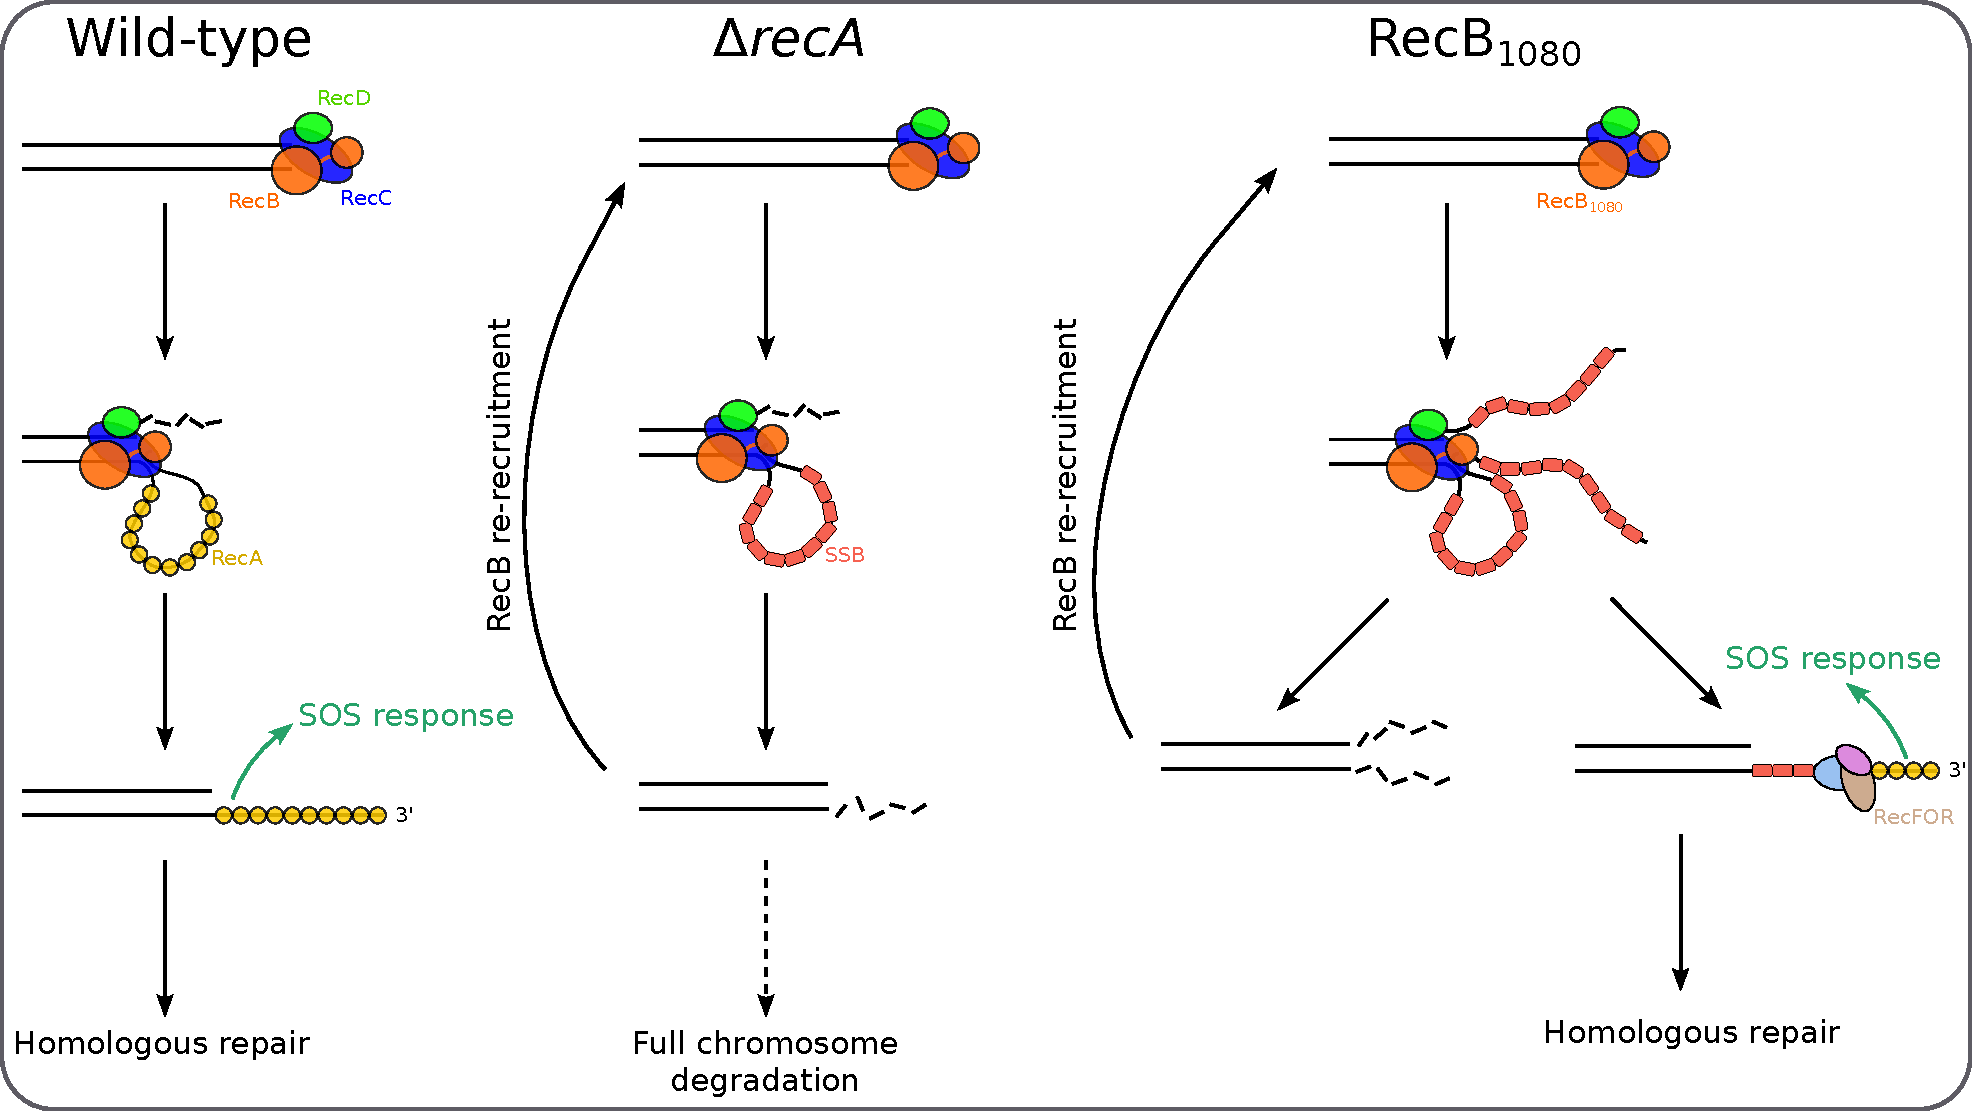
\includegraphics[width=\textwidth]{Figures/Fig_mutants_pathways.pdf}
    \caption{RecBCD recruitment pathways in wild-type \emph{E. coli}, \dreca\ and \teneighty\ mutants. \textbf{(Wild-type)} After DSB recognition, RecBCD degrades DNA until it recognises a Chi-site. It switches activity to create a 3' ssDNA overhang, and promotes RecA loading. The RecA-coated ssDNA can then be used for DNA repair by homologous recombination. \textbf{($\mathbf{\Delta}$reca)} In the absence of RecA, the 3' ssDNA is coated by SSB, and eventually digested by cellular nucleases. Blunting of the DNA end by digestion of the ssDNA creates a new substrate for binding of RecBCD. \textbf{(RecB$\mathbf{_{1080}}$)} Following DSB recognition, \teneighty\ unwinds DNA without digesting it. The unwound ssDNA can either be digested by nucleases, leading to a new blunt dsDNA end and RecBCD re-recruitment; or the RecFOR complex displaces SSB to load RecA, allowing DNA repair by homologous recombination to proceed.}
    \label{Fig:pathways}
\end{figure*}

% Different pathways for RecB recruitment to DSBs in the different mutants
Our observations of cell elongation (Figure \ref{Fig:mutants}A), RecB recruitment to DNA (Figure \ref{Fig:mutants}C), and nucleoid position (Figure \ref{Fig:mutants}D) in the different mutant strains have led us to the model of RecB recruitment described in Figure \ref{Fig:pathways}. In wild-type cells, a DSB is recognised by RecBCD, which promotes RecA loading. The RecA filament triggers the SOS response, and is used for homology search and repair. In the \dreca\ mutant, the 3' ssDNA generated by RecBCD is first coated by SSB, and then degraded by cellular nucleases. This leads to blunting of the DNA end, creating a new substrate on which RecBCD can bind. This circle leads to multiple RecBCD recruitments per DSB, and eventually to full chromosome degradation. In the \teneighty\ mutant, RecBCD unwinds DNA without degrading it. After the ssDNA is coated with SSB, two competing pathways take place: either DNA degradation by nucleases leading to DNA-end blunting and re-recruitment of RecBCD, or displacement of SSB by RecFOR and loading of RecA, leading to SOS induction and homologous repair.